
% ---- fig000_tria.pgf ----
% (c) 2013 Claudio Carboncini - claudio.carboncini@gmail.com
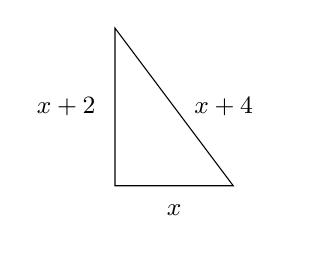
\begin{tikzpicture}[x=10mm,y=10mm,font=\small]
  \draw (1,1) -- (1,3) -- (2.5,1) -- cycle;
  \node [label={[name=label node]left:$x+2$}] at (1,2) {};
  \node [label={[name=label node]left:$x+4$}] at (3,2) {};
  \node [label={[name=label node]below:$x$}] at (1.75,1) {};
\end{tikzpicture}
% -----------------

% ---- fig001_rett.pgf ----
% (c) 2013 Claudio Carboncini - claudio.carboncini@gmail.com
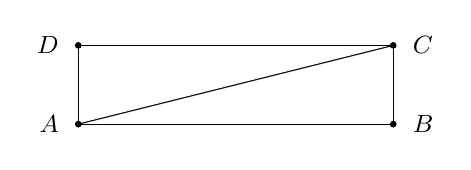
\begin{tikzpicture}[x=10mm,y=10mm,font=\small]
  \draw (1,1) rectangle (5,2);
  \draw (1,1)--(5,2);
  \node [label={[name=label node]left:$A$}] at (1,1) {};
  \node [label={[name=label node]left:$D$}] at (1,2) {};
  \node [label={[name=label node]right:$C$}] at (5,2) {};
  \node [label={[name=label node]right:$B$}] at (5,1) {};

  \foreach \x in {1,5}
    \foreach \y in {1,2}
      \filldraw[fill=black, draw=black]  (\x,\y) circle (1pt);

\end{tikzpicture}
% -----------------

% ---- fig002_seg.pgf ----
% (c) 2013 Claudio Carboncini - claudio.carboncini@gmail.com
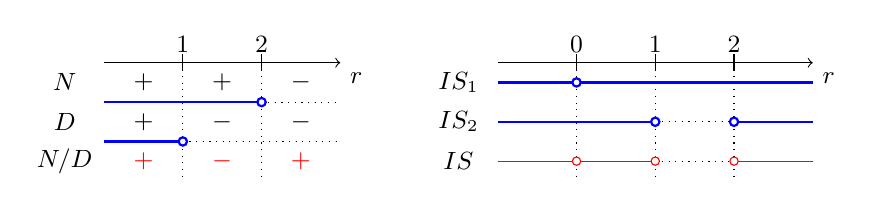
\begin{tikzpicture}[font=\small,x=10mm, y=10mm]

\draw[->] (0,0) -- (3,0) node [below right] () {$r$};
\draw[->] (5,0) -- (9,0) node [below right] () {$r$};

\foreach \x in {1,2,6,7,8}{
\draw(\x,3pt)--(\x,-3pt);
\begin{scope}[dotted]
\draw (\x,0) -- (\x,-1.5);
\draw (2,-.5) -- (3,-.5);
\draw (1,-1) -- (3,-1);
\draw (7,-.75) -- (8,-.75);
\draw (7,-1.25) -- (8,-1.25);
\end{scope}}

\node[above]  at (1,0) {$1$};
\node[above]  at (2,0) {$2$};
\node[above]  at (6,0) {$0$};
\node[above]  at (7,0) {$1$};
\node[above]  at (8,0) {$2$};

\begin{scope}[blue,thick]
\draw (0,-.5) -- (2,-.5);
\draw (1,-1) -- (0,-1);
\draw (5,-.25) -- (6,-.25);
\draw (5,-.25) -- (9,-.25);
\draw (5,-.75) -- (7,-.75);
\draw (8,-.75) -- (9,-.75);

\draw[fill=white] (2,-.5)circle (1.5pt);
\draw[fill=white] (1,-1)circle (1.5pt);
\draw[fill=white] (6,-.25)circle (1.5pt);
\draw[fill=white] (7,-.75)circle (1.5pt);
\draw[fill=white] (8,-.75)circle (1.5pt);
\end{scope}

\foreach \x in {4.5}{
\node  at (\x,-.25) {$IS_1$};
\node  at (\x,-.75) {$IS_2$};
\node  at (\x,-1.25) {$IS$};
}
\foreach \x in {-0.5}{
\node  at (\x,-.25) {$N$};
\node  at (\x,-.75) {$D$};
\node  at (\x,-1.25) {$N/D$};
}

\foreach \z in {.5,1.5}
\node  at (\z,-.25) {$+$};

\foreach \zi in {1.5,2.5}
\node  at (\zi,-.75) {$-$};

\node  at (2.5,-.25) {$-$};
\node  at (0.5,-.75) {$+$};

\begin{scope}[red]
\foreach \y in {-1.25}{
\foreach \ziv in {1.5}
	\node at (\ziv,\y) {$-$};
\foreach \zv in {.5,2.5}
\node at (\zv,\y) {$+$};
\draw (5,-1.25) -- (7,-1.25);
\draw (8,-1.25) -- (9,-1.25);
\draw[fill=white] (6,-1.25)circle (1.5pt);
\draw[fill=white] (7,-1.25)circle (1.5pt);
\draw[fill=white] (8,-1.25)circle (1.5pt);

}
\end{scope}
\end{tikzpicture}
% -----------------

% ---- fig004_tria.pgf ----
% (c) 2013 Claudio Carboncini - claudio.carboncini@gmail.com
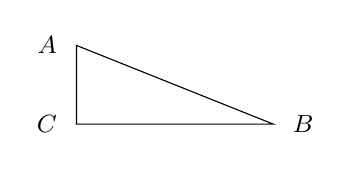
\begin{tikzpicture}[x=10mm,y=10mm,font=\small]

  \draw (1,1) -- (1,2) -- (3.5,1) -- cycle;
  \node [label={[name=label node]left:$A$}] at (1,2) {};
  \node [label={[name=label node]right:$B$}] at (3.5,1) {};
  \node [label={[name=label node]left:$C$}] at (1,1) {};

\end{tikzpicture}
% -----------------

% ---- fig005_trap.pgf ----
% (c) 2013 Claudio Carboncini - claudio.carboncini@gmail.com
\begin{tikzpicture}[x=10mm,y=10mm,font=\small]
  \coordinate(a) at (-2.5,0);
  \coordinate(d) at (120:2.5);
  \coordinate(e) at (90:2.5);
  \coordinate(c) at (60:2.5);
  \coordinate(b) at (2.5,0);
  \coordinate (h) at ($(a)!(c)!(b)$);%trova le coordinate della proiezione di c su a--b
  \draw (-2.5,0) arc (180:0:2.5) -- cycle;% semicirconferenza e diametro
  \draw (a) -- (d) -- (c) -- (b);%disegna il trapezio
  \draw [dotted] (e) -- (0,0);%da E a O
  \draw [dotted] (c) -- (h);% c--h
  \draw [dotted] (e) -- (b);% e--b
  \node [label={[name=label node]below left:$A$}] at (a) {};
  \node [label={[name=label node]below right:$B$}] at (b) {};
  \node [label={[name=label node]above right:$C$}] at (c) {};
  \node [label={[name=label node]above left:$D$}] at (d) {};
  \node [label={[name=label node]above:$E$}] at (e) {};
  \node [label={[name=label node]below:$H$}] at (h) {};
  \filldraw[fill=black, draw=black]  (a) circle (1pt);
  \filldraw[fill=black, draw=black]  (b) circle (1pt);
  \filldraw[fill=black, draw=black]  (c) circle (1pt);
  \filldraw[fill=black, draw=black]  (d) circle (1pt);
  \filldraw[fill=black, draw=black]  (h) circle (1pt);
  \filldraw[fill=black, draw=black]  (e) circle (1pt);

\end{tikzpicture}
% -----------------

% ---- fig006_trap.pgf ----
% (c) 2013 Claudio Carboncini - claudio.carboncini@gmail.com
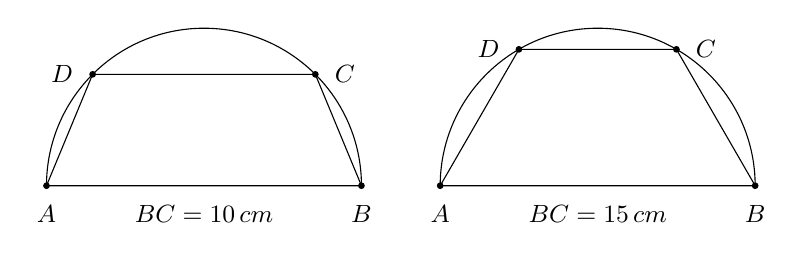
\begin{tikzpicture}[x=10mm,y=10mm,font=\small]
  \coordinate(a) at (-2,0);
  \coordinate(d) at (135:2);
  \coordinate(c) at (45:2);
  \coordinate(b) at (2,0);
  \coordinate(a1) at (3,0);
  \coordinate(d1) at (4,1.732);
  \coordinate(c1) at (6,1.732);
  \coordinate(b1) at (7,0);
  \coordinate(t) at (0,0);
  \coordinate(t1) at (5,0);
  \draw (-2,0) arc (180:0:2) -- cycle;% semicirconferenza e diametro primo trapezio
  \draw (3,0) arc (180:0:2) -- cycle;% semicirconferenza e diametro secondo trapezio
  \draw (a) -- (d) -- (c) -- (b);%disegna il trapezio
  \draw (a1) -- (d1) -- (c1) -- (b1);%disegna il secondo trapezio
  \node [label={[name=label node]below:$A$}] at (a) {};
  \node [label={[name=label node]below:$B$}] at (b) {};
  \node [label={[name=label node]right:$C$}] at (c) {};
  \node [label={[name=label node]left:$D$}] at (d) {};
  \node [label={[name=label node]below:$BC=10\,  cm$}] at (t) {};
  \node [label={[name=label node]below:$A$}] at (a1) {};
  \node [label={[name=label node]below:$B$}] at (b1) {};
  \node [label={[name=label node]right:$C$}] at (c1) {};
  \node [label={[name=label node]left:$D$}] at (d1) {};
  \node [label={[name=label node]below:$BC=15\,  cm$}] at (t1) {};
  \filldraw[fill=black, draw=black]  (a) circle (1pt);
  \filldraw[fill=black, draw=black]  (b) circle (1pt);
  \filldraw[fill=black, draw=black]  (c) circle (1pt);
  \filldraw[fill=black, draw=black]  (d) circle (1pt);
  \filldraw[fill=black, draw=black]  (a1) circle (1pt);
  \filldraw[fill=black, draw=black]  (b1) circle (1pt);
  \filldraw[fill=black, draw=black]  (c1) circle (1pt);
  \filldraw[fill=black, draw=black]  (d1) circle (1pt);

\end{tikzpicture}
% -----------------

% ---- fig007_rett.pgf ----
% (c) 2013 Claudio Carboncini - claudio.carboncini@gmail.com
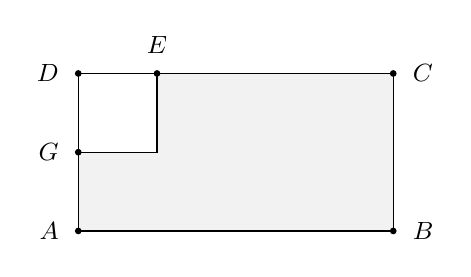
\begin{tikzpicture}[x=10mm,y=10mm,font=\small]

  \fill[fill=gray!10] (1,1) rectangle (5,3);
  \fill[fill=white] (1,3) rectangle (2,2);
  \draw (1,1) rectangle (5,3);
  \draw (1,3) rectangle (2,2);
  \node [label={[name=label node]left:$A$}] at (1,1) {};
  \node [label={[name=label node]left:$D$}] at (1,3) {};
  \node [label={[name=label node]right:$C$}] at (5,3) {};
  \node [label={[name=label node]right:$B$}] at (5,1) {};
  \node [label={[name=label node]left:$G$}] at (1,2) {};
  \node [label={[name=label node]above:$E$}] at (2,3) {};

  \foreach \x in {1,5}
    \foreach \y in {1,3}
      \filldraw[fill=black, draw=black]  (\x,\y) circle (1pt);
      \filldraw[fill=black, draw=black]  (1,2) circle (1pt);
      \filldraw[fill=black, draw=black]  (2,3) circle (1pt);

\end{tikzpicture}
% -----------------

% ---- fig008_rett.pgf ----
% (c) 2013 Claudio Carboncini - claudio.carboncini@gmail.com
\begin{tikzpicture}[x=10mm,y=10mm,font=\small]
  \draw (1,1) rectangle (5,2);
  \draw (1,1)--(2.6,4.4);
  \draw (4.2,1)--(2.6,4.4);
  \draw (2.6,2)--(2.6,4.4);
  \draw [dotted] (2.6,2) -- (2.6,1);
  \node (x) at (4.7,.7) {$x$};
  \node (h) at (2.3,3) {$3x$};
  \node [label={[name=label node]below left:$A$}] at (1,1) {};
  \node [label={[name=label node]above left:$D$}] at (1,2) {};
  \node [label={[name=label node]above right:$C$}] at (5,2) {};
  \node [label={[name=label node]below right:$B$}] at (5,1) {};
  \node [label={[name=label node]below:$E$}] at (4.2,1) {};
  \node [label={[name=label node]above:$F$}] at (2.6,4.4) {};

  \foreach \x in {1,5}
    \foreach \y in {1,2}
      \filldraw[fill=black, draw=black]  (\x,\y) circle (1pt);
      \filldraw[fill=black, draw=black]  (2.6,4.4) circle (1pt);
      \filldraw[fill=black, draw=black]  (4.2,1) circle (1pt);

\end{tikzpicture}
% -----------------

% ---- fig009_quad.pgf ----
% (c) 2013 Claudio Carboncini - claudio.carboncini@gmail.com
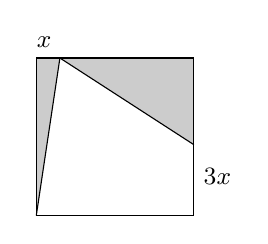
\begin{tikzpicture}[x=10mm,y=10mm,font=\small]

  \fill[fill=gray!40] (1,1) -- (1,3) -- (1.3,3);
  \fill[fill=gray!40] (1.3,3) -- (3,3) -- (3,1.9);
  \draw (1,1) rectangle (3,3);
  \draw (1.3,3)--(1,1);
  \draw (3,1.9)--(1.3,3);
  \node (x) at (1.1,3.2) {$x$};
  \node (h) at (3.3,1.5) {$3x$};

\end{tikzpicture}
% -----------------

% ---- fig010_ango.pgf ----
% (c) 2013 Claudio Carboncini - claudio.carboncini@gmail.com
\begin{tikzpicture}[x=10mm,y=10mm,font=\small]

  \coordinate(v) at (0,0);%il vertice dell'angolo
  \coordinate(a) at (60:4);%la retta a
  \coordinate(b) at (4,0);%la retta b
  \coordinate(a1) at (60:0.8);%il punto A
  \coordinate(b1) at (60:3.2);%il punto B
  \coordinate(p) at (3.2,0);%il punto P
  \coordinate (m) at ($(v)!(b1)!(p)$);%trova le coordinate della proiezione di b su v--p
  \coordinate (n) at ($(v)!(a1)!(p)$);%trova le coordinate della proiezione di b su v--p
  \draw (a) -- (v)  -- (b);%disegna l'angolo
  \draw (b1) -- (p);%disegna il segmento b--p
  \draw (a1) -- (p);%disegna il segmento a--p
  \draw [dotted] (a1) -- (n);%perpendicolare da A a b
  \draw [dotted] (b1) -- (m);%perpendicolare da B a b
  \node [label={[name=label node]left:$V$}] at (v) {};
  \node [label={[name=label node]left:$A$}] at (a1) {};
  \node [label={[name=label node]left:$B$}] at (b1) {};
  \node [label={[name=label node]left:$a$}] at (a) {};
  \node [label={[name=label node]below:$P$}] at (p) {};
  \node [label={[name=label node]below:$M$}] at (m) {};
  \node [label={[name=label node]below:$N$}] at (n) {};
  \node [label={[name=label node]above:$b$}] at (b) {};

\end{tikzpicture}
% -----------------

% ---- fig011_seg.pgf ----
% (c) 2013 Claudio Carboncini - claudio.carboncini@gmail.com
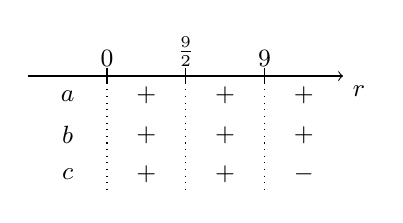
\begin{tikzpicture}[font=\small,x=10mm, y=10mm]

\draw[->] (0,0) -- (4,0) node [below right] () {$r$};

\foreach \x in {1,2,3}{
\draw(\x,3pt)--(\x,-3pt);
\begin{scope}[dotted]
\draw (\x,0) -- (\x,-1.5);
\end{scope}}

\node[above]  at (1,0) {$0$};
\node[above]  at (2,0) {$\frac 9 2$};
\node[above]  at (3,0) {$9$};

\foreach \x in {0.5}{
\node  at (\x,-.25) {$a$};
\node  at (\x,-.75) {$b$};
\node  at (\x,-1.25) {$c$};
}

\foreach \z in {1.5,2.5,3.5}
\node  at (\z,-.25) {$+$};

\foreach \zi in {1.5,2.5,3.5}
\node  at (\zi,-.75) {$+$};

\node  at (1.5,-1.25) {$+$};
\node  at (2.5,-1.25) {$+$};
\node  at (3.5,-1.25) {$-$};
\end{tikzpicture}
% -----------------

% ---- fig012_trap.pgf ----
% (c) 2013 Claudio Carboncini - claudio.carboncini@gmail.com
\begin{tikzpicture}[x=10mm,y=10mm,font=\small]

  \coordinate(a) at (0,2.598);%il punto A
  \coordinate(b) at (0,0);%il punto B
  \coordinate(c) at (4.5,0);%il punto C
  \coordinate(d) at (3,2.598);%il punto D
  \coordinate (h) at ($(a)!(d)!(c)$);%trova le coordinate della proiezione di D su a--c
  \coordinate (h1) at ($(a)!{1/2}!(h)$);
  \coordinate (h2) at ($(h)!{1/2}!(c)$);
  \coordinate (a1) at ($(a)!{1/2}!(d)$);
  \coordinate (d1) at ($(d)!{1/2}!(c)$);
  \draw (a) -- (b)  -- (c) -- (d) -- cycle;%disegna il trapezio
  \draw [] (d) -- (h);%perpendicolare da D a a--c
  \draw [] (a) -- (c);%la diagonale del trapezio
  \draw (h1) node {$//$} ;
  \draw (h2) node {$//$} ;
  \draw (a1) node {$\times$} ;
  \draw (d1) node {$\times$} ;
  \draw (4.1,0.4) node {$\bullet$} ;
  \draw (3.95,0.12) node {$\bullet$} ;
  \node [label={[name=label node]above:$A$}] at (a) {};
  \node [label={[name=label node]below:$B$}] at (b) {};
  \node [label={[name=label node]below:$C$}] at (c) {};
  \node [label={[name=label node]above:$D$}] at (d) {};
  \node [label={[name=label node]below:$H$}] at (h) {};

\end{tikzpicture}
% -----------------

% ---- fig013_cono.pgf ----
% (c) 2013 Claudio Carboncini - claudio.carboncini@gmail.com
\begin{tikzpicture}[x=10mm,y=10mm,font=\small,scale=1.3]

  \coordinate(a) at (0,0);%il punto A
  \coordinate(v1) at (70:5);%il punto V1
  \coordinate(o) at (35:1.5);%il centro del cerchio O
  \coordinate(h) at (1.23,0);%il punto H
  \coordinate (b) at (2.46,0);%il punto B
  \coordinate(v2) at (1.23,6);%il punto v2
  \coordinate (v) at (intersection of a--v1 and h--v2);
  \coordinate (c) at ($(v)!(o)!(b)$);%trova le coordinate della proiezione di o su v--b
  \draw[] (o) circle (0.86);%disegna il cerchio di centro
  \draw[] (v) -- (a) -- (b) -- cycle;%disegna v2--h--a
  \draw[dashed] (v) -- (h);%disegna v--h
  \draw[dashed] (o) -- (c);%disegna o--c
  \draw (h) ellipse (1.23cm and 0.4cm);
  \node [label={[name=label node]above:$V$}] at (v) {};
  \node [label={[name=label node]left:$A$}] at (a) {};
  \node [label={[name=label node]below:$H$}] at (h) {};
  \node [label={[name=label node]right:$B$}] at (b) {};
  \node [label={[name=label node]left:$O$}] at (o) {};
  \node [label={[name=label node]right:$C$}] at (c) {};
\begin{comment}
  \coordinate (h2) at ($(h)!{1/2}!(c)$);
  \coordinate (a1) at ($(a)!{1/2}!(d)$);
  \coordinate (d1) at ($(d)!{1/2}!(c)$);
  \draw (a) -- (b)  -- (c) -- (d) -- cycle;%disegna il trapezio
  \draw [] (d) -- (h);%perpendicolare da D a a--c
  \draw [] (a) -- (c);%la diagonale del trapezio
  \draw (h1) node {$//$} ;
  \draw (h2) node {$//$} ;
  \draw (a1) node {$\times$} ;
  \draw (d1) node {$\times$} ;
  \draw (4.1,0.4) node {$\bullet$} ;
  \draw (3.95,0.12) node {$\bullet$} ;
\end{comment}
\end{tikzpicture}
% -----------------

% ---- fig021_ells.pgf ----
% (c) 2013 Claudio Carboncini - claudio.carboncini@gmail.com
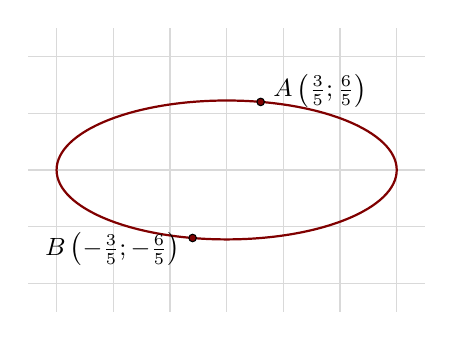
\begin{tikzpicture}[x=8mm, y=8mm,font=\small,scale=.9]
\draw[step=0.8cm,color=gray!30] (-3.5,-2.5) grid (3.5,2.5);
  \tkzInit[xmin=-3.5,xmax=3.5,ymin=-2.5,ymax=2.5]
  \begin{scope}[font=\small]
    \tkzAxeX[below = 3pt]
    \tkzAxeY[left = 1pt]
  \end{scope}
  \tkzFct[domain=-2:2,thick,color=blue]{2*x};

\draw[thick,color=Maroon] (0,0) ellipse (3 and 1.225);
%il punto A
\draw[fill=Maroon] (.6,1.2)circle (1.5pt);
\node[right] at (.65,1.4) {$A \left(\frac{3}{5};\frac{6}{5}\right)$};
%il punto B
\draw[fill=Maroon] (-.6,-1.2)circle (1.5pt);
\node[left] at (-.65,-1.4) {$B \left(-\frac{3}{5};-\frac{6}{5}\right)$};

\end{tikzpicture}
% -----------------

% ---- fig022_prbl.pgf ----
% (c) 2013 Claudio Carboncini - claudio.carboncini@gmail.com
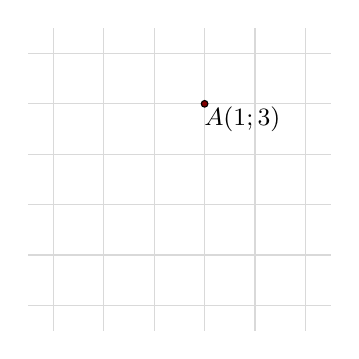
\begin{tikzpicture}[x=8mm, y=8mm,font=\small,scale=.8]
\draw[step=0.8cm,color=gray!30] (-2.5,-1.5) grid (3.5,4.5);
  \tkzInit[xmin=-2.5,xmax=3.5,ymin=-1.5,ymax=4.5]
  \begin{scope}[font=\small]
    \tkzAxeX[below = 3pt]
    \tkzAxeY[left = 1pt]
  \end{scope}
\tkzFct[domain=-.5:3.5,thick,color=Maroon]{-x*x+3*x+1};
\tkzFct[domain=-3.5:6.5,thick,color=blue]{x+2};
%il punto A
\node[right] at (0.8,2.7) {$A (1;3)$};
\draw[fill=Maroon] (1,3)circle (1.5pt);
\end{tikzpicture}
% -----------------

% ---- fig023_crch.pgf ----
% (c) 2013 Claudio Carboncini - claudio.carboncini@gmail.com
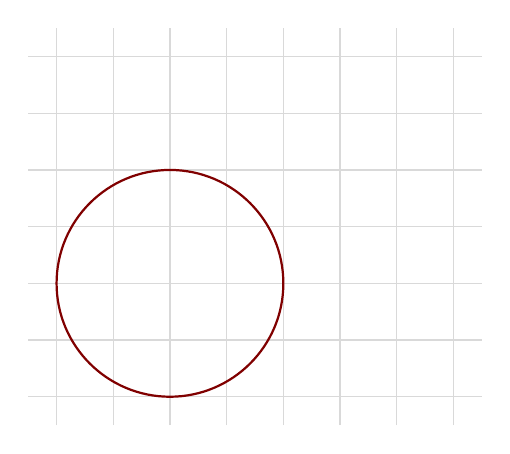
\begin{tikzpicture}[x=8mm, y=8mm,font=\small,scale=.9]
\draw[step=0.8cm,color=gray!30] (-2.5,-2.5) grid (5.5,4.5);
  \tkzInit[xmin=-2.5,xmax=5,ymin=-2.5,ymax=4]
  \begin{scope}[font=\small]
    \tkzAxeX[below = 3pt]
    \tkzAxeY[left = 1pt]
  \end{scope}
\tkzFct[domain=-3:5.5,thick,color=blue]{-0.75*x+3};

\draw[thick,color=Maroon] (0,0) circle (2);
\end{tikzpicture}
% -----------------

% ---- fig024_tutte.pgf ----
% (c) 2013 Claudio Carboncini - claudio.carboncini@gmail.com
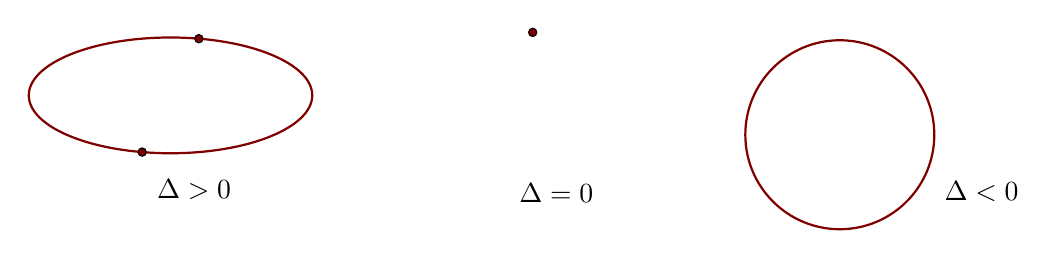
\begin{tikzpicture}[x=6mm, y=6mm]
  \tkzInit[xmin=-3.5,xmax=3.5,ymin=-2.5,ymax=2.5]
  \tkzFct[domain=-2:2,thick,color=blue]{2*x};
\draw[thick,color=Maroon] (0,0) ellipse (3 and 1.225);
\draw[fill=Maroon] (.6,1.2)circle (1.5pt);
\draw[fill=Maroon] (-.6,-1.2)circle (1.5pt);
\node[color =black] at (.5,-2) {$\Delta>0$};

\begin{scope}[xshift=4cm,yshift=-1cm]
\tkzInit[xmin=-2.5,xmax=3.5,ymin=-1.5,ymax=4.5]
\tkzFct[domain=-.5:3.5,thick,color=Maroon]{-x*x+3*x+1};
\tkzFct[domain=-3.5:6.5,thick,color=blue]{x+2};
\draw[fill=Maroon] (1,3)circle (1.5pt);
\node[color =black] at (1.5,-0.4) {$\Delta=0$};
\end{scope}

\begin{scope}[xshift=8.5cm,yshift=-.5cm]
\tkzInit[xmin=-2.5,xmax=5,ymin=-2.5,ymax=4];
\tkzFct[domain=-3:5.5,thick,color=blue]{-0.75*x+3};
\draw[thick,color=Maroon] (0,0) circle (2);
\node[color =black] at (3,-1.2) {$\Delta<0$};
\end{scope}


\end{tikzpicture}
% -----------------

% ---- fig025_iprb.pgf ----
% (c) 2013 Claudio Carboncini - claudio.carboncini@gmail.com

\begin{tikzpicture}[x=6mm, y=6mm,font=\small,scale=.7]
\draw[step=0.6cm,color=gray!30] (-4.5,-4.5) grid (4.5,4.5);
  \tkzInit[xmin=-4.5,xmax=4.5,ymin=-4.5,ymax=4.5]
  \begin{scope}[font=\small]
    \tkzAxeX[below = 3pt]
    \tkzAxeY[left = 1pt]
  \end{scope}
    \tkzFct[domain=-4.5:4.5,thick,color=blue]{x};
    \tkzFct[domain=-4.5:4.5,very thick,color=Maroon]{-x};
\end{tikzpicture}
% -----------------

% ---- fig026_iprb.pgf ----
% (c) 2013 Claudio Carboncini - claudio.carboncini@gmail.com
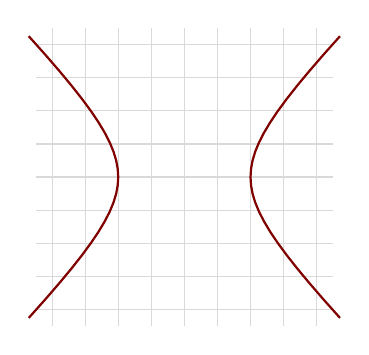
\begin{tikzpicture}[x=6mm, y=6mm,font=\small,scale=.7]
\draw[step=0.6cm,color=gray!30] (-4.5,-4.5) grid (4.5,4.5);
  \tkzInit[xmin=-4.5,xmax=4.5,ymin=-4.5,ymax=4.5]
  \begin{scope}[font=\small]
    \tkzAxeX[below = 3pt]
    \tkzAxeY[left = 1pt]
  \end{scope}
   \pgfmathsetmacro{\e}{1.41421}   % eccentricity
    \pgfmathsetmacro{\a}{2}
    \pgfmathsetmacro{\b}{(\a*sqrt((\e)^2-1)} 
    \draw[thick,color=Maroon] plot[domain=-1.5:1.5] ({\a*cosh(\x)},{\b*sinh(\x)});
    \draw[thick,color=Maroon] plot[domain=-1.5:1.5] ({-\a*cosh(\x)},{\b*sinh(\x)});
    \tkzFct[domain=-4:4,thick,color=blue]{-1.5*x};
\end{tikzpicture}
% -----------------

% ---- fig027_iprb.pgf ----
% (c) 2013 Claudio Carboncini - claudio.carboncini@gmail.com
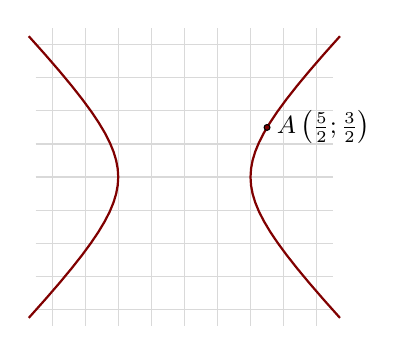
\begin{tikzpicture}[x=6mm, y=6mm,font=\small,scale=.7]
\draw[step=0.6cm,color=gray!30] (-4.5,-4.5) grid (4.5,4.5);
  \tkzInit[xmin=-4.5,xmax=4.5,ymin=-4.5,ymax=4.5]
  \begin{scope}[font=\small]
    \tkzAxeX[below = 3pt]
    \tkzAxeY[left = 1pt]
  \end{scope}
   \pgfmathsetmacro{\e}{1.41421}   % eccentricity
    \pgfmathsetmacro{\a}{2}
    \pgfmathsetmacro{\b}{(\a*sqrt((\e)^2-1)} 
    \draw[thick,color=Maroon] plot[domain=-1.5:1.5] ({\a*cosh(\x)},{\b*sinh(\x)});
    \draw[thick,color=Maroon] plot[domain=-1.5:1.5] ({-\a*cosh(\x)},{\b*sinh(\x)});
    \tkzFct[domain=-4:5,thick,color=blue]{x-1};
    \node[right] at (2.5,1.5) {$A \left(\frac 5 2;\frac 3 2\right)$};
    \draw[fill=Maroon] (2.5,1.5)circle (1.5pt);
\end{tikzpicture}
% -----------------

% ---- fig028_iprb.pgf ----
% (c) 2013 Claudio Carboncini - claudio.carboncini@gmail.com
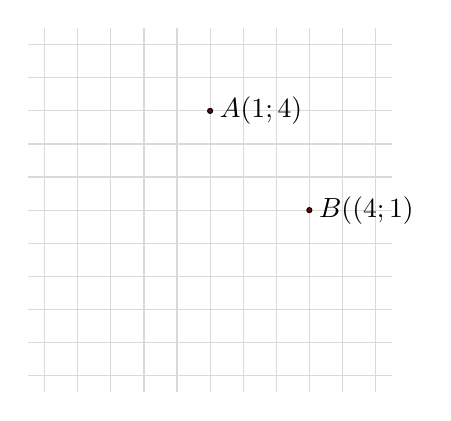
\begin{tikzpicture}[x=7mm, y=7mm, scale=.6]
\draw[step=0.7cm,color=gray!30] (-4.5,-4.5) grid (6.5,6.5);
  \tkzInit[xmin=-4,xmax=6,ymin=-4,ymax=6]
  \begin{scope}[font=\small]
    \tkzAxeX[below = 3pt]
    \tkzAxeY[left = 1pt]
  \end{scope}
  \tkzFct[domain=-5.5:0,thick,color=Maroon]{4/x}
  \tkzFct[domain=-0:5.5,thick,color=Maroon]{4/x}
\tkzFct[domain=-2:6,thick,color=blue]{-x+5};
 \draw[fill=Maroon] (1,4)circle (1.5pt);
\node[right] at (1,4) {$A (1;4)$};
\draw[fill=Maroon] (4,1)circle (1.5pt);
\node[right] at (4,1) {$B ((4;1)$};

\end{tikzpicture}
% -----------------

% ---- fig029_iprb.pgf ----
% (c) 2013 Claudio Carboncini - claudio.carboncini@gmail.com

\begin{tikzpicture}[x=7mm, y=7mm, scale=.6]
\draw[step=0.7cm,color=gray!30] (-4.5,-4.5) grid (4.5,4.5);
  \tkzInit[xmin=-4.5,xmax=4.5,ymin=-4.5,ymax=4.5]
  \begin{scope}[font=\small]
    \tkzAxeX[below = 3pt]
    \tkzAxeY[left = 1pt]
  \end{scope}
  \tkzFct[domain=-4.5:0,thick,color=Maroon]{1/x}
  \tkzFct[domain=-0:4.5,thick,color=Maroon]{1/x}
\tkzFct[domain=-3:4,thick,color=blue]{-x+1};
\end{tikzpicture}
% -----------------

% ---- fig030_iprb.pgf ----
% (c) 2013 Claudio Carboncini - claudio.carboncini@gmail.com
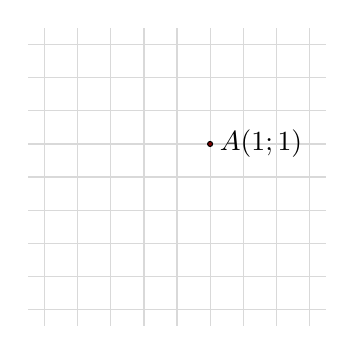
\begin{tikzpicture}[x=7mm, y=7mm, scale=.6]
\draw[step=0.7cm,color=gray!30] (-4.5,-4.5) grid (4.5,4.5);
  \tkzInit[xmin=-4.5,xmax=4.5,ymin=-4.5,ymax=4.5]
  \begin{scope}[font=\small]
    \tkzAxeX[below = 3pt]
    \tkzAxeY[left = 1pt]
  \end{scope}
  \tkzFct[domain=-4.5:0,thick,color=Maroon]{1/x}
  \tkzFct[domain=-0:4.5,thick,color=Maroon]{1/x}
\tkzFct[domain=-3:4,thick,color=blue]{-x+2};
\draw[fill=Maroon] (1,1)circle (1.5pt);
 \node[right] at (1,1) {$A (1;1)$};
\end{tikzpicture}
% -----------------

% ---- fig031_trap.pgf ----
% (c) 2013 Claudio Carboncini - claudio.carboncini@gmail.com
\begin{tikzpicture}[x=10mm,y=10mm,font=\small]
  \coordinate(a) at (-2.5,0);
  \coordinate(d) at (130:2.5);
  \coordinate(e) at (90:2.5);
  \coordinate(c) at (50:2.5);
  \coordinate(b) at (2.5,0);
  \coordinate(o) at (0,0);
  \coordinate (h) at ($(a)!(c)!(b)$);%trova le coordinate della proiezione di c su a--b
  \coordinate (k) at ($(d)!(e)!(c)$);%trova le coordinate della proiezione di e su d--c
  \fill[color=gray!20](o)--(k)--(c);
  \fill[color=gray!20](h)--(b)--(c);
  \draw (-2.5,0) arc (180:0:2.5) -- cycle;% semicirconferenza e diametro
  \draw (a) -- (d) -- (c) -- (b);%disegna il trapezio
  \draw [dashdotted] (e) -- (0,0);%da E a O
  \draw [dotted] (c) -- (h);% c--h
 \draw [dotted] (o) -- (c);% o--c
  \node [label={[name=label node]below left:$A$}] at (a) {};
  \node [label={[name=label node]below right:$B$}] at (b) {};
  \node [label={[name=label node]above right:$C$}] at (c) {};
  \node [label={[name=label node]above left:$D$}] at (d) {};
  \node [label={[name=label node]above:$E$}] at (e) {};
  \node [label={[name=label node]below:$H$}] at (h) {};
  \node [label={[name=label node]below left:$K$}] at (k) {};
  \node [label={[name=label node]below:$O$}] at (o) {};
  \node[] at (2.1,-.3) {$\frac{25-y}2$};
  \node[] at (25:2.4) {$x$};
  \node[] at (70:2.25) {$\frac y 2$};
  \node[] at (45:1.25) {$\frac {25} 2$};
  \filldraw[fill=black, draw=black]  (a) circle (1pt);
  \filldraw[fill=black, draw=black]  (b) circle (1pt);
  \filldraw[fill=black, draw=black]  (c) circle (1pt);
  \filldraw[fill=black, draw=black]  (d) circle (1pt);
  \filldraw[fill=black, draw=black]  (h) circle (1pt);
  \filldraw[fill=black, draw=black]  (e) circle (1pt);
  \filldraw[fill=black, draw=black]  (k) circle (1pt);
  \filldraw[fill=black, draw=black]  (o) circle (1pt);

\end{tikzpicture}
% -----------------

% ---- fig051_rufi.pgf ----
% (c) 2013 Claudio Carboncini - claudio.carboncini@gmail.com

\begin{tikzpicture}[x=5mm,y=5mm]
\matrix (a)[matrix of nodes, nodes in empty cells,nodes={ text width=8mm, text depth=1mm, text centered}]{
&$1$&$-7$&$4$&$ 12 $\\
$ -1 $&&$ -1 $&$ 8 $&$-12$\\
&$ 1 $&$ -8 $&$12$&//\\
};  
\begin{scope}[blue]
\draw(a-1-2.north west)--(a-3-1.south east);
\draw(a-2-1.south west)--(a-2-5.south east);
\draw(a-1-4.north east)--(a-3-4.south east);
      \end{scope}
\end{tikzpicture}
% -----------------
